\section{Pruebas preliminares}

\begin{figure}
    \centering
    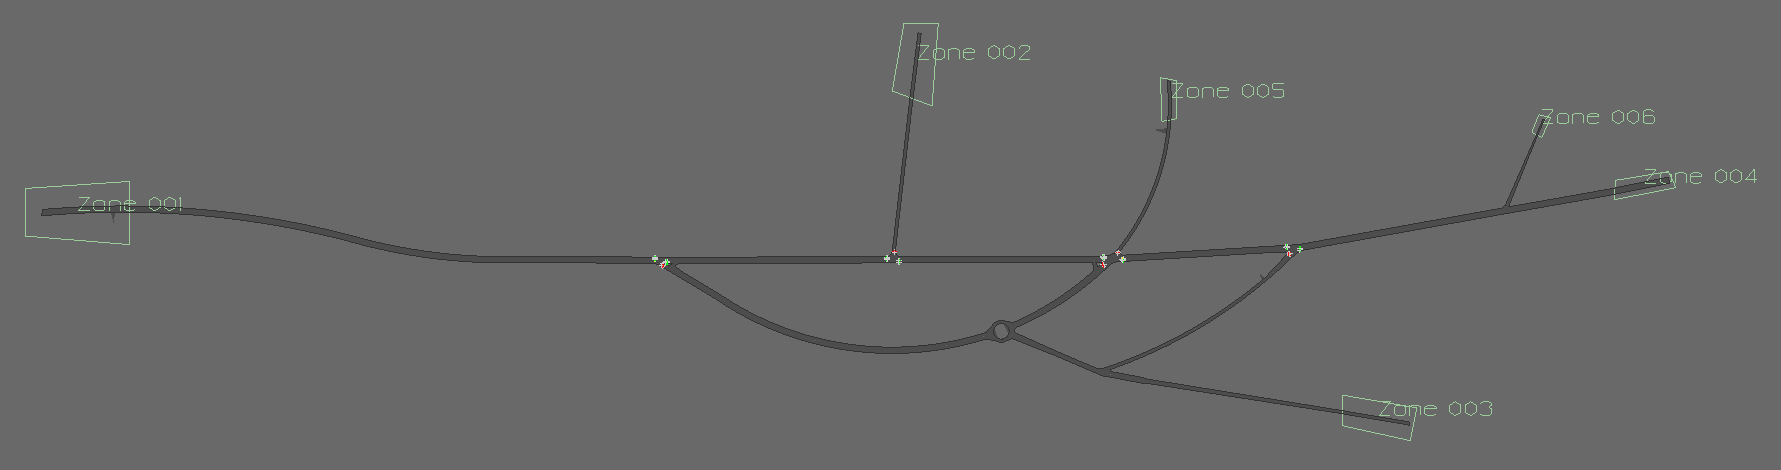
\includegraphics[width=\linewidth]{figuras/network8.png}
    \caption{Red de transporte utilizada para las pruebas preliminares.}
    \label{fig:network8}
\end{figure}

La validación preliminar del \emph{framework} se realizó utilizando la implementación de TraCI en Python incluída en la distribución de SUMO. Esta consiste en una librería para Python 2.7+ y 3.0+, la cual implementa un cliente TraCI en su totalidad (\autocite{pytraci, pytracisrc}), permitiendo así la validación del correcto funcionamiento de los comandos implementados en el \emph{framework} PVeins.

Por otro lado, la red de transporte utilizada para las pruebas corresponde a una red simple, incluida por defecto en la instalación de Paramics. Esta red consiste en un corredor central y conjunto de calles que lo intersectan (ver figura \ref{fig:network8}). El flujo de vehículos en la red es medio-bajo, manteniéndose bajo los 500 vehículos activos en toda la red en cualquier momento dado.

A lo largo del desarrollo de este trabajo, se utilizó la librería anteriormente mencionada, junto con el entorno de \emph{debugging} de Visual Studio y la red de transporte, para probar la correcta implementación de cada funcionalidad que se le agregó al \emph{framework}. Se implementaron simples \emph{scripts} en Python para probar cada una de las funcionalidades desarrolladas; sólo se utilizará uno de éstos como ejemplo a continuación, ya que no es factible ni interesante exponer todas las pruebas realizadas en este documento, dada la gran cantidad de éstas que se efectuaron y el alto grado de similitud que existe entre las mismas.

Además, implementado ya el \emph{framework} en su totalidad, se realizaron pruebas de validación de mayor envergadura, midiendo la eficiencia y la efectividad del sistema para la simulación de grandes redes de transporte. Los resultados de éstas pruebas se presentan en el capítulo \ref{cap:validacion}.

\subsection{Ejemplo de script de prueba: cambio de ruta}

\begin{figure}
    \centering
    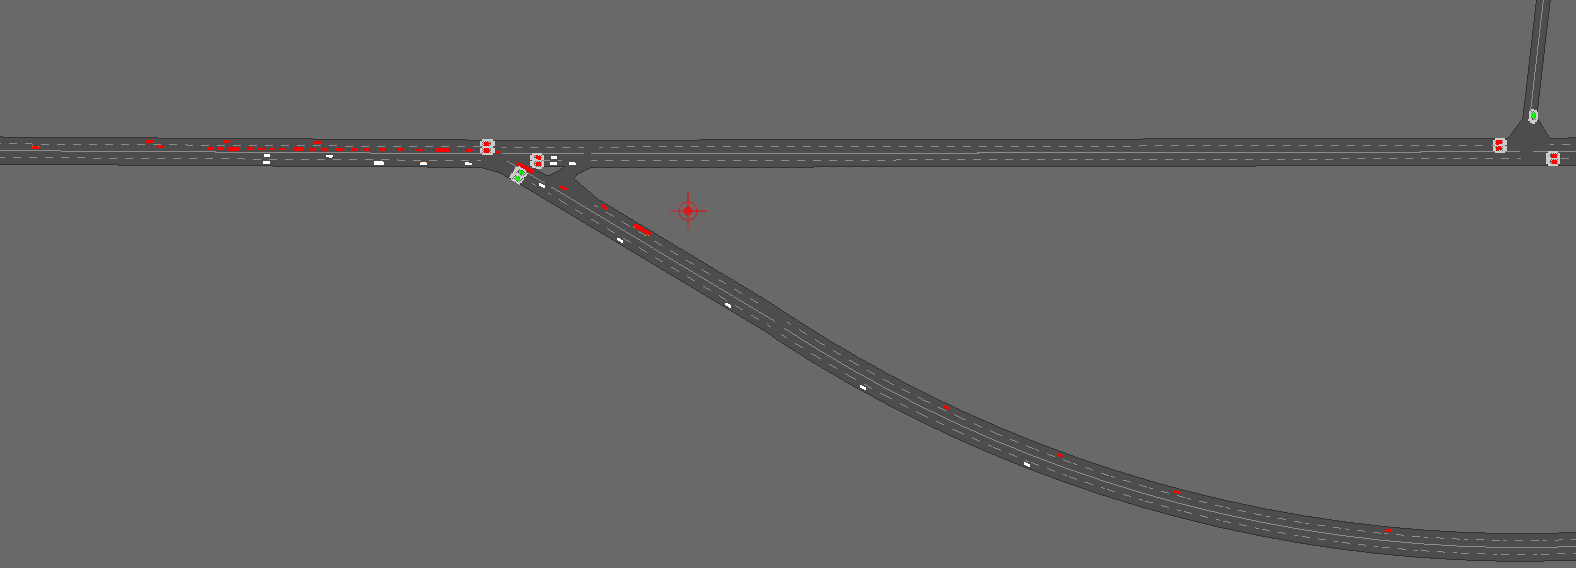
\includegraphics[width=\linewidth]{figuras/network8_routechange.png}
    \caption{Visualización del \emph{test} de cambio de ruta en curso. Los vehículos pintados de rojo son aquellos afectados por el cambio.}
    \label{fig:network8:routechange}
\end{figure}

El código \ref{code:py_routechange} expone el \emph{script} utilizado para una prueba de la funcionalidad del cambio de ruta en TraCI, la cual fue implementada en la última etapa de desarrollo del software por lo que ya se contaba con una base con más funcionalidades sobre la cual construir (\emph{e.g.}, obtención de valores mediante suscripciones).

El procedimiento es simple; el \emph{script} avanza la simulación en un \emph{loop}, obteniendo luego de cada iteración la lista de vehículos en la red. De estos vehículos, encuentra aquellos que se encuentran en la primera calle de una ruta predefinida y procede a cambiar su ruta original por una nueva, al mismo tiempo pintándolos de un color rojo para poder distinguirlos del resto. El resultado puede observarse en la figura \ref{fig:network8:routechange}.

Este código expone de manera clara la estructura del \emph{loop} de simulación TraCI, estructura que se replica en VEINS (aunque de manera mucho más compleja); el cliente es quien controla la ejecución de los pasos de simulación, avanzando el escenario a medida que va realizando sus propios cálculos y análisis. También demuestra las razones por la cual se llevó a cabo el desarrollo en etapas comentado en la sección \ref{sec:metodologia} -- si bien el enfoque de esta prueba es la funcionalidad de cambio de ruta, es necesario también el uso de otras funcionalidades de TraCI como el \emph{handshake} de inicio de conexión (\texttt{traci.init(\dots)}), la suscripción a variables de vehículo (\texttt{traci.vehicle.subscribe(\dots)} y \texttt{.getSubscriptionResults(\dots)}), el avance de la simulación (\texttt{traci.simulationStep()}) y la obtención de variables de vehículo (\texttt{traci.getRoadID(\dots)}).

\begin{figure*}
    \begin{minipage}{\linewidth}
        \lstinputlisting[style=MyPython, caption={\emph{Script} para la prueba de cambio de ruta.}, label={code:py_routechange}]{codigo/pytraci_routechange.py}
    \end{minipage}
\end{figure*}

